\documentclass[letterpaper]{article}

\usepackage{natbib,alifeconf}  %% The order is important

\usepackage{hyperref}

\usepackage{subcaption}

\usepackage{hhline}

\usepackage{multirow}

\usepackage{rotating}

\ifdefined\mydraft
\mydraft
\fi

\graphicspath{{img/}}

\newcommand{\STAB}[1]{\begin{tabular}{@{}c@{}}#1\end{tabular}}

% *****************
%  Requirements:
% *****************
%
% - All pages sized consistently at 8.5 x 11 inches (US letter size).
% - PDF length <= 8 pages for full papers, <=2 pages for extended
%    abstracts.
% - Abstract length <= 250 words.
% - No visible crop marks.
% - Images at no greater than 300 dpi, scaled at 100%.
% - Embedded open type fonts only.
% - All layers flattened.
% - No attachments.
% - All desired links active in the files.

% Note that the PDF file must not exceed 5 MB if it is to be indexed
% by Google Scholar. Additional information about Google Scholar
% can be found here:
% http://www.google.com/intl/en/scholar/inclusion.html.


% If your system does not generate letter format documents by default,
% you can use the following workflow:
% latex example
% bibtex example
% latex example ; latex example
% dvips -o example.ps -t letterSize example.dvi
% ps2pdf example.ps example.pdf


% For pdflatex users:
% The alifeconf style file loads the "graphicx" package, and
% this may lead some users of pdflatex to experience problems.
% These can be fixed by editing the alifeconf.sty file to specify:
% \usepackage[pdftex]{graphicx}
%   instead of
% \usepackage{graphicx}.
% The PDF output generated by pdflatex should match the required
% specifications and obviously the dvips and ps2pdf steps become
% unnecessary.


% Note:  Some laser printers have a serious problem printing TeX
% output. The use of ps type I fonts should avoid this problem.


\title{TODO SignalGP Dishtiny}
\author{Matthew Andres Moreno$^{1}$ \\
\mbox{}\\
$^1$BEACON Center, Michigan State University, East Lansing, MI 48824 \\
mmore500@msu.edu} % email of corresponding author

% For several authors from the same institution use the same number to
% refer to one address.
%
% If the names do not fit well on one line use
%         Author 1, Author 2 ... \\ {\Large\bf Author n} ...\\ ...
%
% If the title and author information do not fit in the area
% allocated, place \setlength\titlebox{<new height>} after the
% \documentclass line where <new height> is 2.25in



\begin{document}
\maketitle

\begin{abstract}

Natural evolutionary history is profoundly shaped by evolutionary transitions in individuality, episodes where independent replicating entities united to form more complex replicating entities.
Fraternal transitions in individuality occur specifically when the derived replicating entity is composed of kin groups of a lower-level replicator;
examples include the evolution of multicellularity and the evolution of eusocial insect colonies.
The conditions necessary for fraternal transitions to occur and the mechanisms by which such transitions occur have been a fruitful target of scientific interest and open questions that warrant continued investigation remain.

In previous work, we developed a digital framework to study fraternal transitions of individuality.
This framework, DISHTINY, is designed as distributed system: individual digital cells operate independently and periodically communicate with neighbors via messages.
This project uses DISHTINY to investigate the relationship between mutation intensity and the evolution of cooperation.
Specifically, we ask
\begin{itemize}
\item Do cooperative strategies become disadvantageous under higher mutation intensity?
\item What is the relationship between group size and the effect of mutation intensity on the viability of cooperative strategies?
\end{itemize}

We find that high mutational load derails the evolution of cooperative, multicellular phenotypes.
Specifically, we observed,
\begin{itemize}
\item cooperative reproductive behavior observed under low mutational load is replaced by antagonistic reproductive behavior under high mutational load,
\item cooperative resource sharing behavior observed under low mutational load disappears under higher mutational loads,
\item cooperative reproductive behavior and cooperative resource sharing exhibit opposite trends in sensitivity mutational intensity with respect to group size, the first being more sensitive in large groups and the latter being more sensitive in small groups.
\end{itemize}
\end{abstract}


\section{Introduction}

In a fraternal evolutionary transition of individuality, a new, more complex replicating entity is derived from the combination of cooperating kin which have entwined their long-term fates \citep{west2015major}.
Eusocial insect colonies and multicellular organisms exemplify this phenomenon  \citep{smith1997major}.
In the first case, individual insects (e.g., ants) act in concert towards the subsistence and propagation of the collective (e.g., an ant colony).
In the second, individual cells join together into a highly structured collective in which only a fraction participate in the germ line.

A meta-organism composed of fraternal kin (e.g., a multicellular organism composed of individual cells) in some ways resembles a distributed system.
In order for a meta-organism to succeed, its constituent parts --- which interact asynchronously --- must cooperate to perform tasks and make decisions at the collective level.
For example, ants use pheromones to exchange information about the location and quality of food sources in order to collectively explore their environment and forage resources for the colony.

Distributed systems must contend with failures and, ideally, nevertheless continue to function effectively.
The most commonly considered failure mode is crash failures, where an element of the distributed system loses some functionality or becomes unresponsive.
However, failure modes where a node begins to exhibit arbitrary, or even malicious, behavior --- referred to as byzantine failures --- are also possible.
Like distributed systems, fraternal groups contend with failures of their constituent members.
Over time, an individual member accumulates mutations which, eventually, may cause that member to cease to function properly (i.e., a crash failure) or even act maliciously (i.e., a byzantine failure).
In particular, multicellular organisms often contend with cancer, a byzantine failure where tumor cells engage in unchecked reproduction.
Studying the relationship between mutation and fraternal transitions of individuality is of both scientific and practical interest.
From a scientific perspective, we might gain insight into the mutation-management challenges that fraternal groups face and the evolutionary trajectories that clear those hurdles.
From a practical perspective, better understanding evolved mutation-management solutions in fraternal groups may provide inspiration for new methods to secure distributed systems against failures.

In previous work, we have developed a digital framework to study fraternal transitions of individuality \cite{moreno2018toward}.
This framework, DISHTINY, is designed as distributed system: individual digital cells operate independently and periodically communicate with neighbors via messages.
This project uses DISHTINY to investigate the relationship between mutation intensity and the evolution of cooperation.
Specifically, we ask
\begin{itemize}
\item Do cooperative strategies become disadvantageous under higher mutation intensity?
\item What is the relationship between group size and the effect of mutation intensity on the viability of cooperative strategies?
\end{itemize}


\section{Methods}

In order to demonstrate that the DISHTINY platform selects for detectable hierarchical transitions in individuality, we performed experiments where cell-like organisms evolved parameters to control manually-designed strategies such as resource-sharing, reproductive decision-making, and apoptosis.
We will first cover the design of the DISHTINY platform and then describe the simple cell-like organisms we used to evaluate the platform.

\subsection{DISHTINY}

\begin{figure*}[t]
\begin{center}
\includegraphics[width=2.0\columnwidth]{img/explanatory}
\caption{
\textbf{Activation signaling, and net resource collection for three different-sized same-channel networks during a resource wave event.}
At the top, a resource wave is depicted propagating over three updates and then ceasing for four updates (left to right).
In row $a$, a small two-cell channel-signaling group (far left, in green) is activated; tracking the resource wave (top) yields a small net resource harvest (far right).
In row $b$, an intermediate-sized 13-cell channel-signaling group yields a high net resource harvest.
Finally, in row $c$, a large 29-cell channel-signaling group incurs a net negative resource harvest.
In rows $a$, $b$, and $c$, dark purple indicates the active state, light purple indicates the quiescent state, and white indicates the ready state.
}
\label{fig:explanatory}
\end{center}
\end{figure*}


DISHTINY allows cell-like organisms to replicate across a toroidal grid.
Over discrete timesteps (``updates''), the cells can collect a continuous-valued resource.
Once sufficient resource has been accrued, cells may pay $3.0$ resource to place a daughter cell on an adjoining tile of the toroidal grid (i.e., reproduce), replacing any existing cell already there.
As cells reproduce, they can choose to include offspring in the parent's cooperating ``signaling channel'' group or force offspring to create a new cooperating ``signaling channel'' group.

As shown at the top of Figure \ref{fig:explanatory}, resources appear at a single point then spread outwards update-by-update in a diamond-shaped wave, disappearing when the expanding wave reaches a predefined limit.
Cells must be in a costly ``activated'' state to collect resource as it passes.
The cell at the starting position of a resource wave is automatically activated, and will send the activate signal to neighboring cells on the same signaling channel.
The newly activated cells, in turn, activate their own neighbors registered to the same signaling channel.
Neighbors registered to other signaling channels do not activate.
Each cell, after sending the activation signal, enters a temporary quiescent state so as not to reactivate from the signal.
In this manner, cells sharing a signaling channel activate in concert with the expanding resource wave.
As shown Figure \ref{fig:explanatory}$a,b$, the rate of resource collection for a cell is determined by the size and shape of of its same-channel signaling network;
small or fragmented same-channel signaling networks will frequently miss out on resource as it passes by.

Each cell pays a resource cost when it activates.
This cost is outweighed by the resource collected such that cells that activate in concert with a resource wave derive a net benefit.
Recall, though, that resource waves have a limited extent.
Cells that activate outside the extent of a resource wave or activate out of sync with the resource wave (due to an indirect path from the cell that originated the signal) pay the activation cost but collect no resource.
Cells that frequently activate erroneously use up their resource and die.
In our implementation, organisms that accrue a resource debt of $-5$ or greater are killed.
This erroneous activation scenario is depicted in Figure \ref{fig:explanatory}$c$.

In this manner, ``Goldilocks'' --- not to small and not too big --- signaling networks are selected for.
Based on a randomly chosen starting location, resource wave starting points (seeds) are tiled over the toroidal grid such that the extents of the resource waves touch, but do not overlap.
All waves start and proceed synchronously;
when they complete, the next resource waves are seeded.
This process ensures that selection for ``Goldilocks'' same-channel signaling networks is uniformly distributed over the toroidal grid.

Cells control the size and shape of their same-channel signaling group through strategic reproduction.
Three choices are afforded: whether to reproduce at all, where among the four adjoining tiles of the toroidal grid to place their offspring, and whether the offspring should be registered to the parent's signaling channel or be given a random channel ID (in the range 1 to $2^{64}$).
The probability of channel collision is miniscule: $60 \times 60 \times 50100$ (the grid dimensions times the number of simulation updates) independent channel values will only collide with probability $1 \times 10^{-11}$.
No guarantees are made about the uniqueness of a newly-generated channel ID, but chance collisions are rare.

To ensure turnover of channel groups, a channel generation limit is enforced.
Each time a cell spawns a daughter cell sharing the same channel, the parent's channel generation counter is incremented and the daughter cell's channel generation counter is then initialized to match their  parent's counter.
Once the channel generation counter reaches a limit, in this implementation defined as the resource wave radius, daughter cells may no longer be endowed with the parent's channel ID; a new, randomly-drawn channel ID is assigned to daughter cells instead.

Hierarchical levels are introduced into the system through multiple separate, but overlaid, instantiations of this resource wave/channel-signaling scheme.
We refer to each independent resource wave/channel-signaling system as a ``level.''
In our experiments, we allowed two resource wave/channel-signaling levels, identified here as level one and level two.
On level one, resource waves extended a radius of three toroidal tiles.
On level two they extended a radius of 24 toroidal tiles.
On both levels, activated cells netted $+1.0$ resource from a resource wave, but suffered an activation penalty of $-5.0$ if no resource was available.
Due to the different radii of resource waves on different levels, level one selects for small same-channel signaling networks and level two selects for large same-channel signaling networks.

Cells were marked with two separate channel IDs, one for level one and another for level two.
We enforced hierarchical nesting of same-channel signaling networks during reproduction:
daughter cells may inherit neither channel ID, just the level-two channel ID, or both channel IDs.
Daughter cells may not inherit only the level-one channel ID while having a different level-two channel ID.
The distribution of IDs across the level-two and level-one channels can be envisioned by analogy to political countries and territories.
Each country (i.e., level-two channel network) may have one or many territories (i.e., level-one channel network).
However, no territory spans more than one country.
Figure \ref{fig:outcome_grids} depicts hierarchically nested channel states at the end of three evolutionary runs.

Channel IDs enable straightforward detection of an evolutionary transition in individuality.
Because common channel IDs may only arise systematically through inheritance, common channel IDs indicate a close hereditary relationship in addition to a close cooperative relationship.
Because new channel IDs arise first in a single cell, same-channel signaling networks are reproductively bottlenecked, ensuring meaningful reproductive lineages at the level of the same-channel signaling network.
To recognize an evolutionary transition in individuality, we therefore evaluate
\begin{enumerate}
\item Do cells with the same channel ID choose to share resources (e.g., cooperate)?
\item Is there division of reproductive labor between members of the same channel (e.g., do cells at the interior of a network cede reproduction to those at the periphery?)
\end{enumerate}
If these conditions are met among cells sharing the same level-one channel, a first-level transition in individuality may have occurred.
Likewise, if these conditions are met among cells sharing the same level-two channel, a second-level transition in individuality may have occurred.
In either case, observation of altruistic behavior, such as an apoptosis response to mutation, would further evidence a transition.

\subsection{Organisms}

\begin{figure*}[t]
\begin{center}
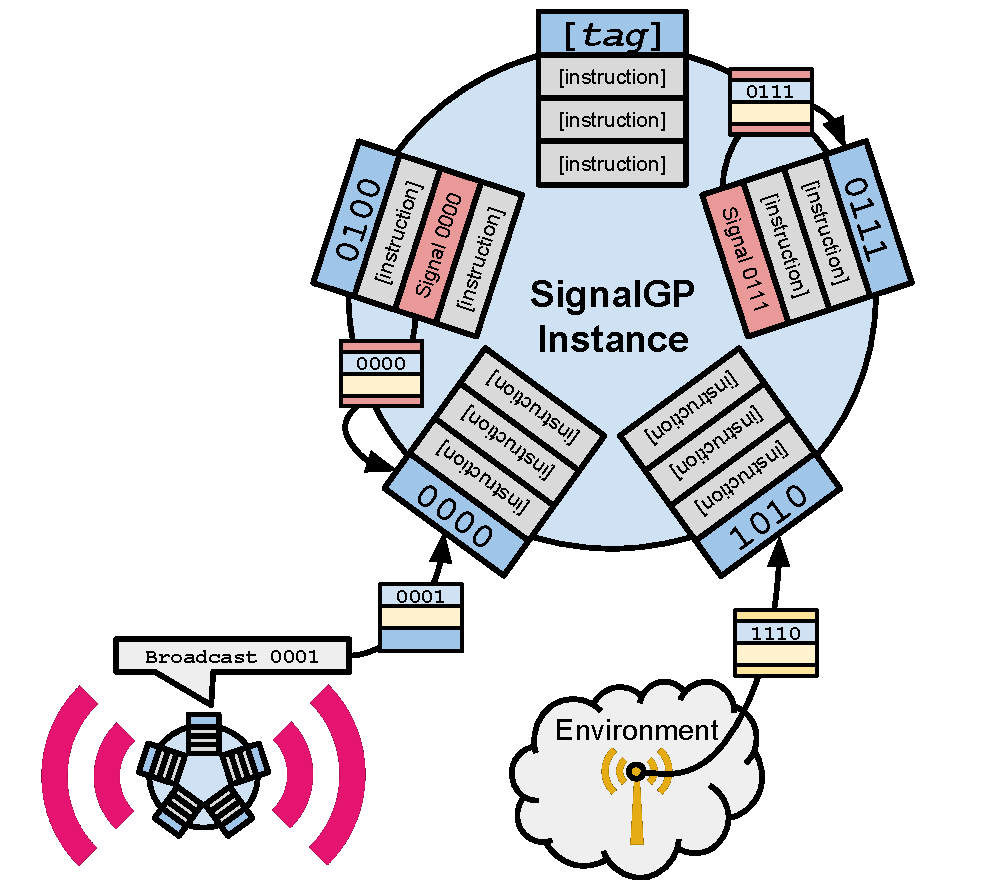
\includegraphics[width=\columnwidth]{img/signalgp-cartoon}%
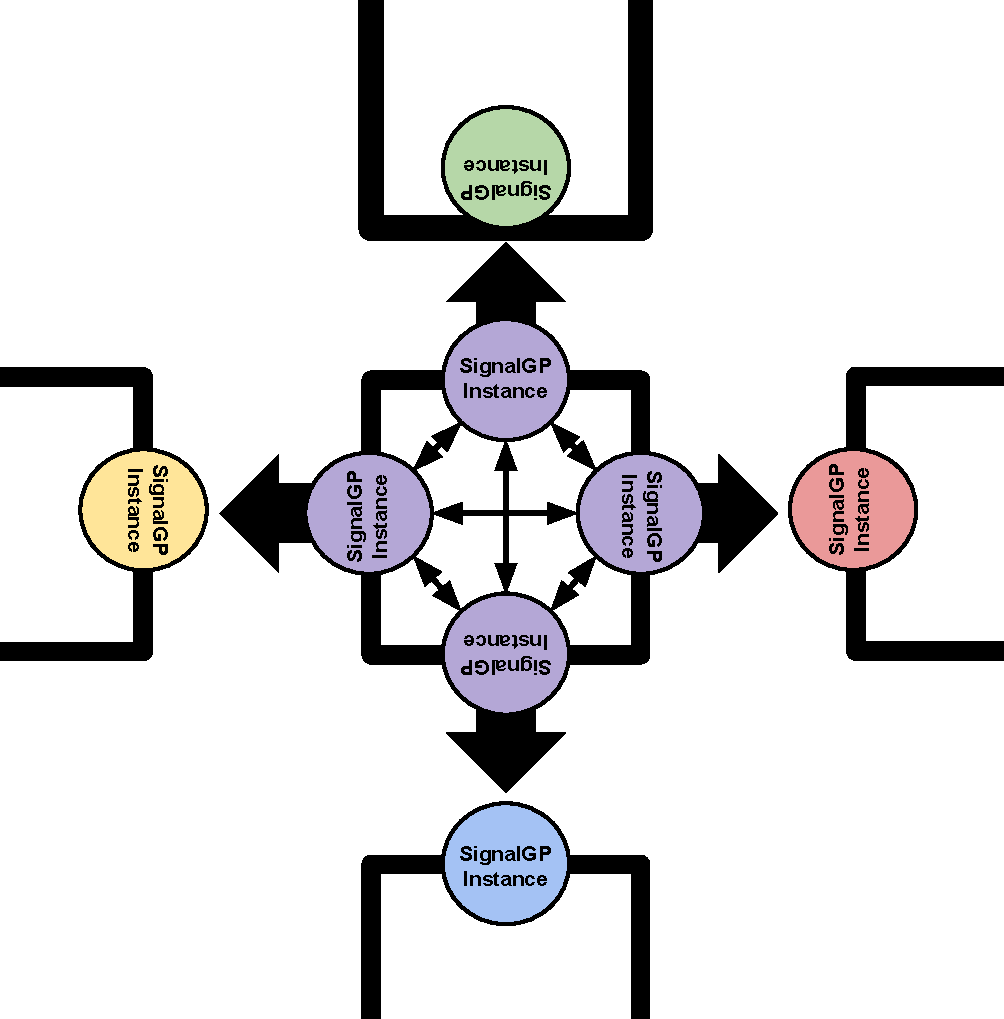
\includegraphics[width=\columnwidth]{img/dishtinygp-cartoon}
\caption{TODO}
\label{fig:signalgp-dishtinygp}
\end{center}
\end{figure*}


We performed our experiments using cell-level organisms based on SignalGP \cite{lalejini2018evolving}.
These cell-level organisms are in no way inherent to the DISHTINY platform, but were merely developed to study the platform.

In order to ensure symmetry
unlike previous work on grid-based cooperation

A combination of event-driven and procedural sensing.

\subsection{Instruction Library}

In addition to the generic arithmetic, logic, and program flow instructions in the default SignalGP instruction set, which is detailed in \cite{lalejini2018evolving}, we define the following instructions.
Instructions that involve an extracellular neighbor default to the cell that the executing SignalGP instance is facing, but may be modified by a register-based argument.
Many instructions in the listing are provided in several variants, which are detailed in the accompanying description.

\begin{itemize}
\item \textbf{RNG Draw}
Draw a random value between 0.0 and 1.0 from on board random number generator and store result in register.
\item \textbf{Send/Broadcast Intracellular Message}
Send a message to a single other SignalGP instance within the cell or to all SignalGP instances (except the executing instance) within the current cell.
\item \textbf{Set Stockpile Reserve}
Mark twice the amount of resource as ineligible for sharing.
The amount may be modified by a register-based argument.
\item \textbf{Activate/Deactivate Intercellular Inbox}
Mark or unmark the intercellular inbox in a particular direction to refuse incoming messages.
At cell birth, the inbox is deactivated.
\item \textbf{Share Resource}
Send a proportion of the cell's stockpiled resource to a neighboring cell.
One instruction defaults to sending a large proportion of available resource (50\%) to the neighboring cell.
A second instruction defaults to sending a small proportion of available resource (5\%) to the neighboring cell.
The proportion of available resource can be adjusted by a register-based argument.
\item \textbf{Accept/Decline Sharing}
Mark the cell to decline resource sent by neighbors.
Declined resource is retained by the sending cell (with no resource lost).
Regardless of this instruction, cells with negative resource stockpiles automatically decline shared resource.
At birth, the cell is marked to accept sharing.
\item \textbf{Send/Broadcast Intercellular Message}
Send a message to a single cellular neighbor or to all cellular neighbors.
\item \textbf{Reproduce}
Attempt to spawn a child cell in a particular direction, paid for out of the parent cell's resource stockpile.
If sufficient resource is not available in the cell's stockpile, no resource is action is taken.
Variants of this instruction are defined for each channel ID inheritance level: from endowing the daughter cell with the parental channel IDs across all levels, to endowing the daughter cell with a new level-one channel ID but the parent's level-two channel ID, to endowing the daughter cell with all-new channel IDs.
If a channel generation counter limit has been reached, reproduction is simply attempted at the next highest level; even with channel generation counters maxed out, cells may generate offspring with all-new channel IDs.
\item \textbf{Pause Reproduction}
Pause cellular reproduction in a single direction for the remainder of the current update and for the entire next update.
Variants of this instruction pause reproduction at a certain wave/channel-signaling level or across all channel ID inheritance levels.
\item \textbf{Increase Channel Generation Counter}
Increases the cell's channel generation counter by one.
The amount the cell's generation counter is increased by can be adjusted by register-based argument.
\item \textbf{Apoptosis}
The cell is killed at the end of the current update.
Two variants are defined.
Under the conplete variant, the cell's channel ID partial and complete
\item \textbf{Designate/Revoke Heir} apoptosis 80\% of reproduction cost and own stockpile amount
\item \textbf{Query Own Stockpile}
Sets a designated register to the amount of resource present in the cell's stockpile.
\item \textbf{Query Own Channel Generation Counter} -Lev
This instruction sets a designated register to the value of the cell's channel generation counter.
A variant of this instruction is provided for each wave/channel-signaling level.
\item \textbf{Query Is Neighbor Live}
This instruction sets a designated register to 1 if the neighboring tile contains a live cell and 0 otherwise.
\item \textbf{Query Is Neighbor Channel Set}
This instruction sets a designated register to 1 if the neighboring tile contains active channel IDs and 0 otherwise.
\item \textbf{Query Is Neighbor My Cellular Child}
This instruction sets a designated register to 1 if the neighboring cell is the daughter of the querying cell and 0 otherwise.
\item \textbf{Query Is Neighbor My Cellular Parent}
This instruction sets a designated register to 1 if the neighboring cell is the parent of the querying cell and 0 otherwise.
\item \textbf{Query Does Neighbor's Channel ID Match Mine}
This instruction sets a designated register to 1 if the neighboring cell has the same channel ID as the querying cell and 0 otherwise.
A variant of this instruction is provided for each wave/channel-signaling level.
\item \textbf{Query Does Neighbor's Channel ID Descend From Mine}
This instruction sets a designated register to 1 if the neighboring cell's highest-level channel ID is different from the querying cell's highest-level channel ID, but is descended from the querying cell's channel ID.
This instruction allows a querying cell to sense whether its neighbor is a member of a same-channel group that is a propagule of the querying cell's same-channel group.
\item \textbf{Query Does My Channel ID Descend From Neighbor's}
This instruction sets a designated register to 1 if the querying cell's highest-level channel ID is different from the neighboring cell's highest-level channel ID, but is descended from the neighboring cell's channel ID.
\item \textbf{Query Neighbor's Channel ID}
This instruction sets a designated register to the neighbor's channel ID.
\item \textbf{Query Neighbor's Stockpile}
This instruction sets a designated register to the amount of resource present in the neighbor's stockpile.
\end{itemize}

\subsection{Event Library}

The activating affinity of each event is set at the outset of each experiment using a pseudo random number generator.

\begin{itemize}
\item \textbf{On Update}
This event is triggered at the outset of each simulation update.
\item \textbf{Facing Cellular Child}
This event is triggered at the outset of an update if the SignalGP instance is facing a neighboring cell that is the querying cell's daughter.
\item \textbf{Stockpile Debt}
This event is triggered at the outset of an update if the amount of resource in a cell's stockpile is negative.
\item \textbf{Neighbor's Channel ID Matches Mine} defined per level
This event is triggered at the outset of an update if a SignalGP instance is facing a neighbor cell that shares its channel ID.
A different event is provided for each resource wave/channel-signaling level.
\item \textbf{Neighbor's Channel ID Descends From Mine}
This event is triggered at the outset of an update if the neighboring cell's highest-level channel ID is different from the querying cell's highest-level channel ID, but is descended from the querying cell's channel ID.
This event allows a querying cell to sense whether its neighbor is a member of a same-channel group that is a propagule of the querying cell's same-channel group.
\end{itemize}

\subsection{Treatments}

Three experimental parameters:
\begin{enumerate}
\item hierarchy (and wave size)
\item resource distribution (wave vs even)
\item recognize/sense channels (as proxy for kin)
\end{enumerate}

We performed six treatments with these combinations of experimental parameters
\begin{enumerate}
\item treat=resource-even\_channelsense-no\_nlev-two
\item treat=resource-wave\_channelsense-no\_nlev-two
\item treat=resource-wave\_channelsense-yes\_nlev-onesmall
\item treat=resource-even\_channelsense-yes\_nlev-two
\item treat=resource-wave\_channelsense-yes\_nlev-onebig
\item treat=resource-wave\_channelsense-yes\_nlev-two
\end{enumerate}

\subsection{Implementation}

We implemented our experimental system using the Empirical library for scientific software development in C++, available at \url{https://github.com/devosoft/Empirical}.
The code used to perform and analyze our experiments, our figures, data from our experiments, and a live in-browser demo of our system is available via the Open Science Framework at \url{https://osf.io/g58xk/}.


\section{Results and Discussion}

In DISHTINY, cellular reproduction is contingent on resource collection and cellular decision-making (e.g., to execute the ``Reproduce'' instruction) and is not directly tied to the elapsing of updates.
So, although each replicate ran for the same number of updates, the number of cellular generations elapsed differs between replicates.
Indeed, because cellular reproduction is asynchronous, extant cells within a single replicate differ with respect to number of cellular generations removed from an initial seed cell.
However, computing the mean across extant cells for cellular generations elapsed at the end of a run provides a reasonable notion of phylogenetic depth.

\begin{table}
 \centering
 \begin{tabular}{l c|cc} % alignment of each column data
 \multicolumn{4}{c}{\textbf{Elapsed Cellular Generations}} \\
 & & \multicolumn{2}{c}{Resource Wave Size} \\
 & & Small & Large \\
 \hline
 \multirow{5}{*}{\STAB{\rotatebox[origin=c]{90}{\parbox{1.5cm}{\centering Mutational\\Load}}}} & 1 & $298 \pm 234$ & $50 \pm 38$ \\
 & 2 & $224 \pm 145$ & $32 \pm 10$ \\
 & 3 & $111 \pm 22$ & $17 \pm 3$
 \\
 & 4 & $74 \pm 11$ & $11 \pm 1$ \\
 & 5 & $120 \pm 2$ & $6 \pm 1$ \\
\end{tabular}
\caption{
Number of elapsed cellular generations by treatment (mean $\pm$ standard deviation across replicates).
}
\label{tab:cell_generations}
\end{table}


Table \ref{tab:cell_generations} shows mean cellular generations elapsed at the end of an evolutionary run for each treatment.
The number of elapsed cellular generations varies systematically across treatments, generally deceasing both with increasing mutational load and increased resource wave size.
Across treatments, elapsed cellular generation counts range from around 298 to around 6.

Large resource wave size may depress the cellular generation rate for two reasons.
Because of their reduced radius and duration, in our implementation small resource wave events occur more densely and more frequently.
Although each small resource wave dispenses less resource compared to large resource wave, the small resource wave replicates enjoy greater average resource availability per update.
In addition, forming the small same-channel groups required to fully exploit small resource waves is a less challenging task than forming the large same-channel groups required to fully exploit large resource waves.

There are also two reasons why mutational load may depress the cellular generation rate.
First, because mutations cause some proportion of reproduction events to result in dead offspring (e.g., offspring that execute an ``Apoptosis'' instruction) or sterile offspring (e.g., offspring that fail to execute the ``Reproduce'' instruction ), higher mutational load may inherently depress the growth rate of the population.
Second, higher mutational load may make developing and maintaining cooperative same-channel resource collection groups more difficult, therefore suppressing the resource collection rate.
For example, under greater mutational load same-channel resource collection groups may have to contend with members that unnecessarily expend resource replacing existing members with their offspring instead of growing the group, disrupt the group by inserting offspring with a new channel ID at the interior of the group, or hog resource that may otherwise be shared between group members.

\begin{figure}[!htbp]
\begin{center}
\rotatebox{90}{~~~~~Mutational Load 1}
\begin{subfigure}[b]{0.45\columnwidth}
  \centering
  Small Resource Wave\\~\\
  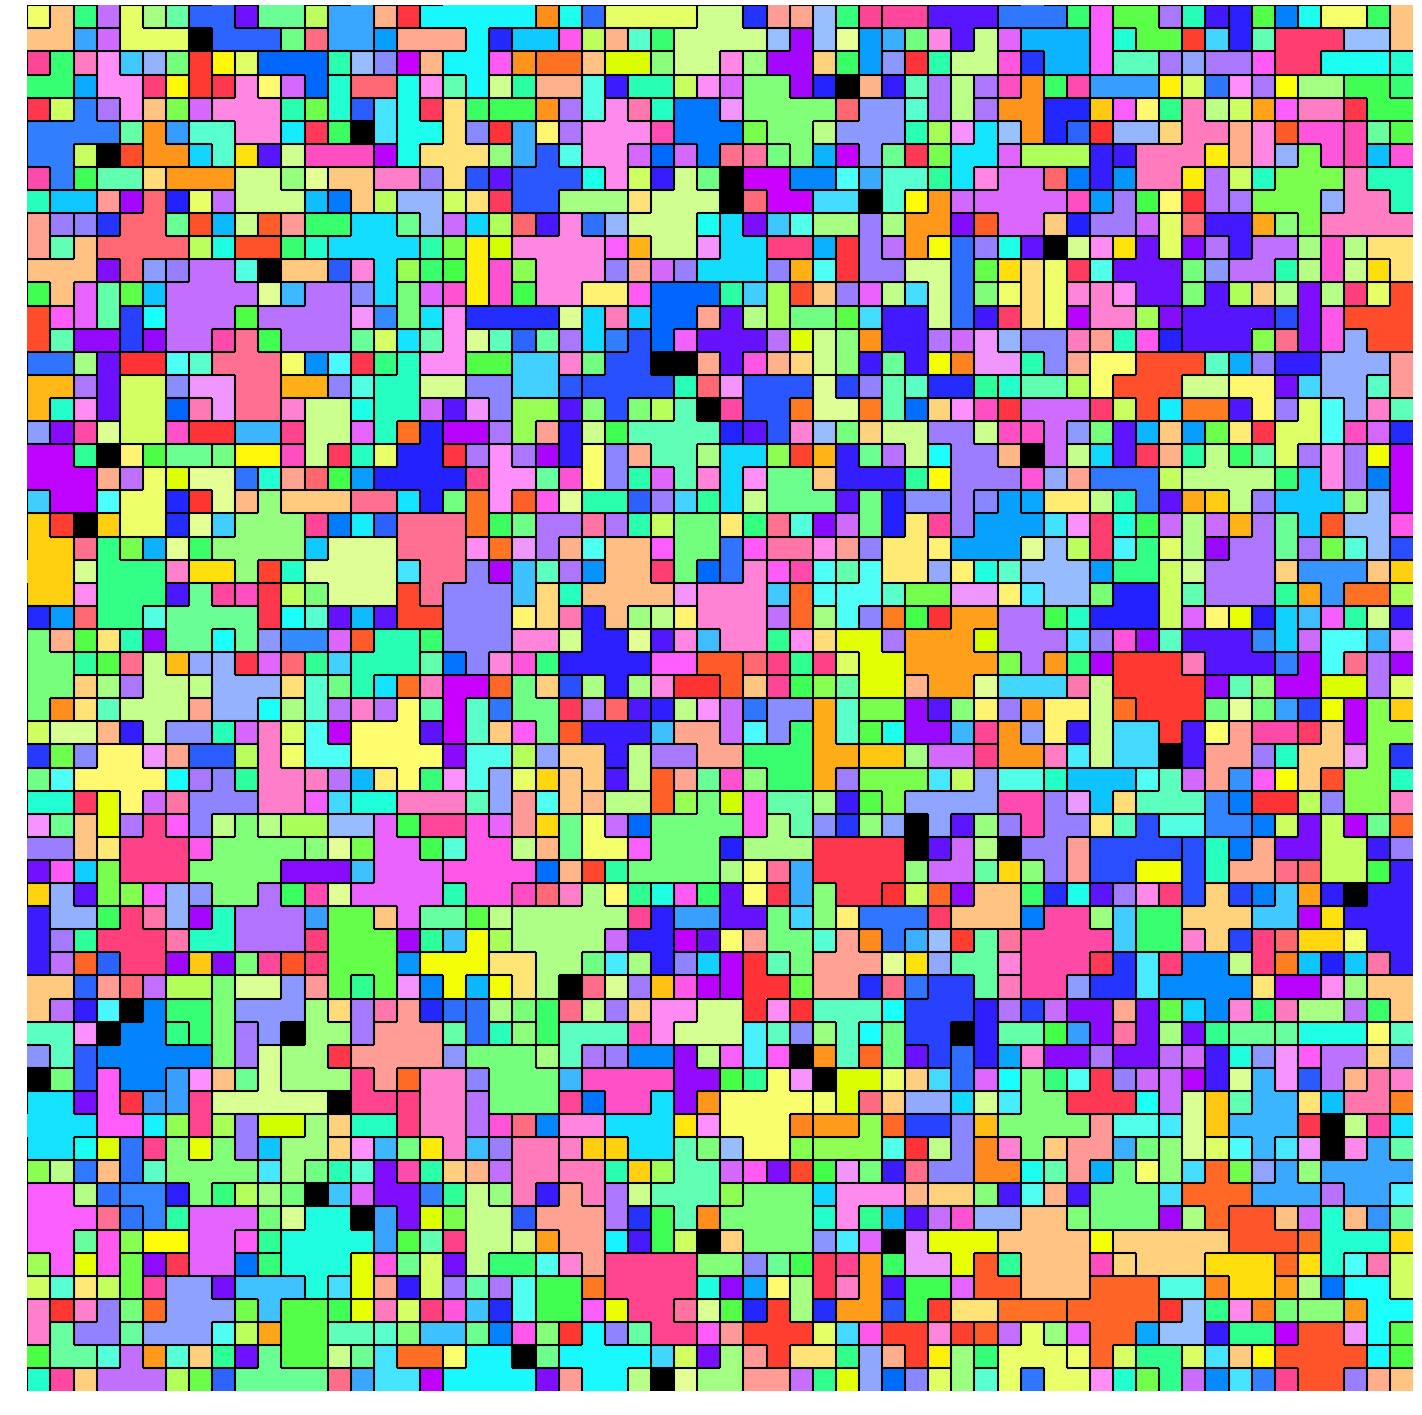
\includegraphics[width=\columnwidth]{seed=1001+title=channel_viz+treat=wave-small__mut-a_low+update=50000+_data_hathash_hash=38f284fb779ed3f5+_script_fullcat_hash=474b4115ecde8750+_source_hash=d53f428-clean+ext=}
\end{subfigure}
\begin{subfigure}[b]{0.45\columnwidth}
  \centering
  Large Resource Wave\\~\\
  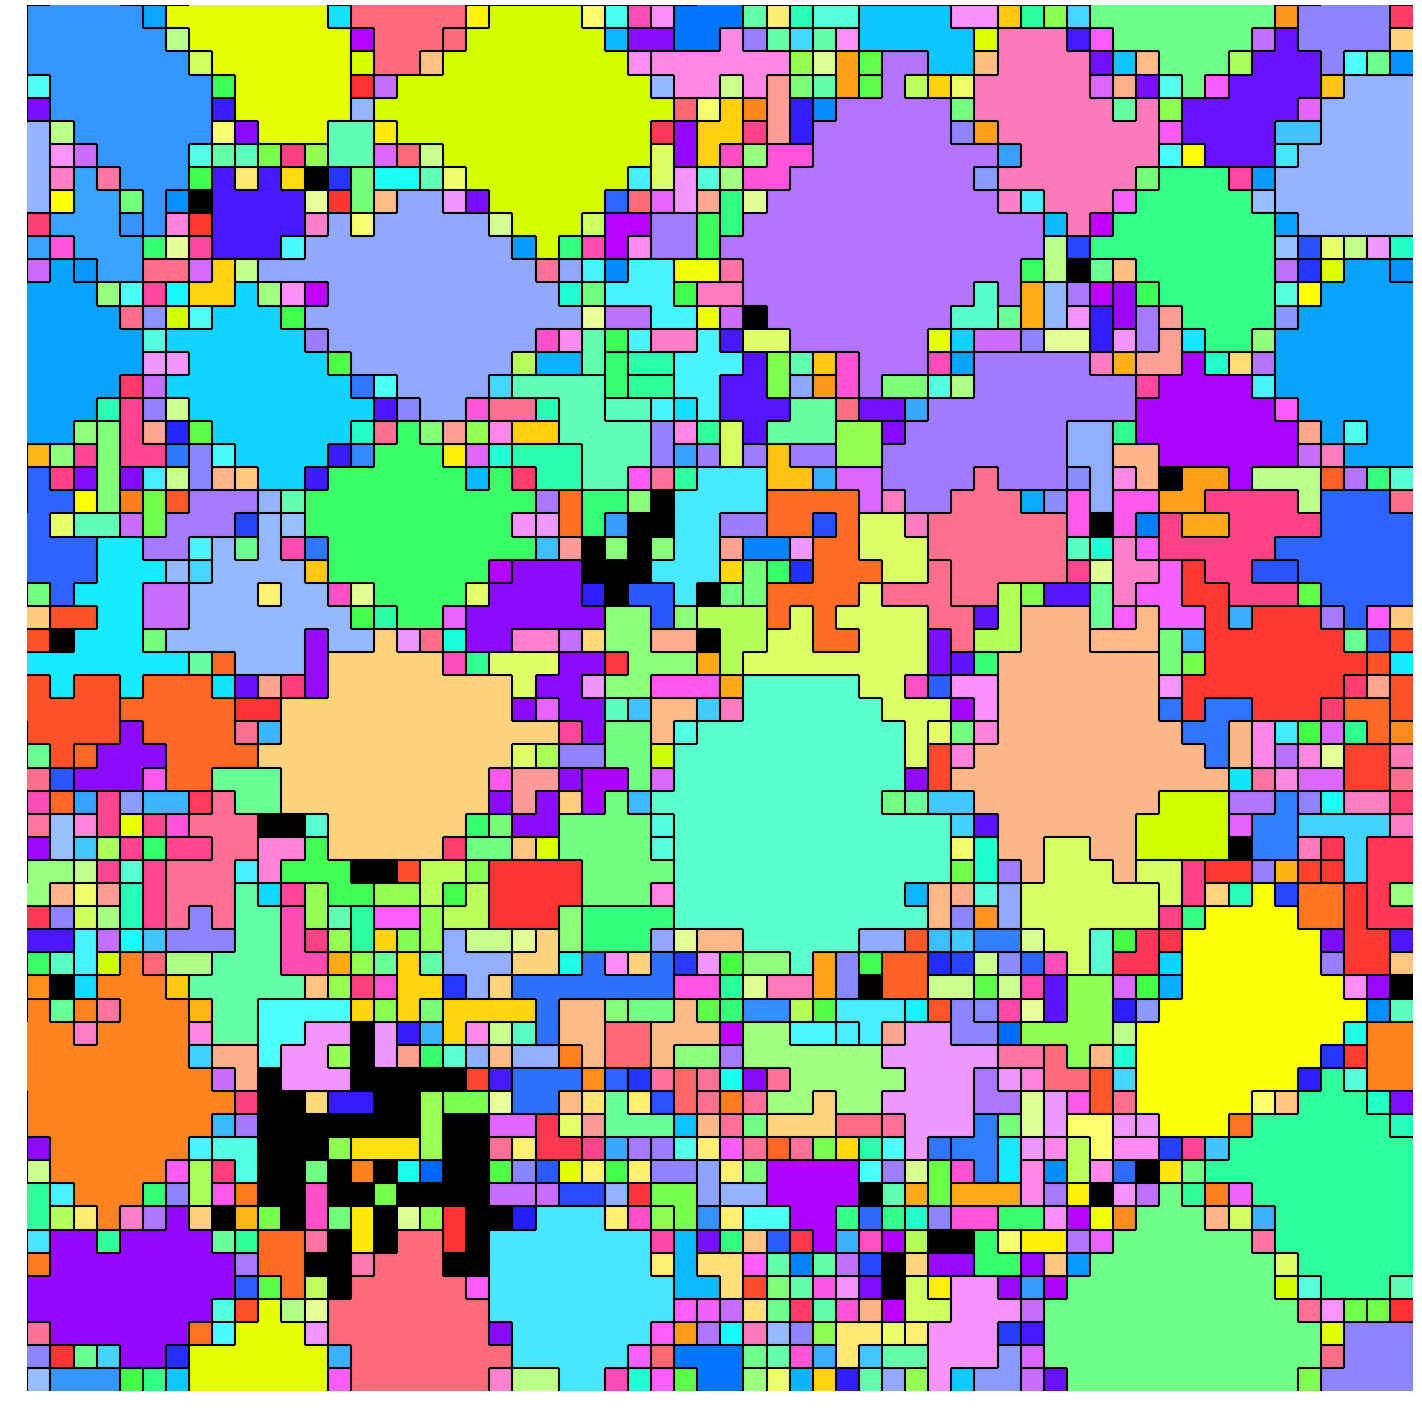
\includegraphics[width=\columnwidth]{seed=1001+title=channel_viz+treat=wave-big__mut-a_low+update=50000+_data_hathash_hash=33ac6f19e90e7ab9+_script_fullcat_hash=474b4115ecde8750+_source_hash=d53f428-clean+ext=}
\end{subfigure}

\rotatebox{90}{~~~~~~~Mutational Load 2}
\begin{subfigure}[b]{0.45\columnwidth}
  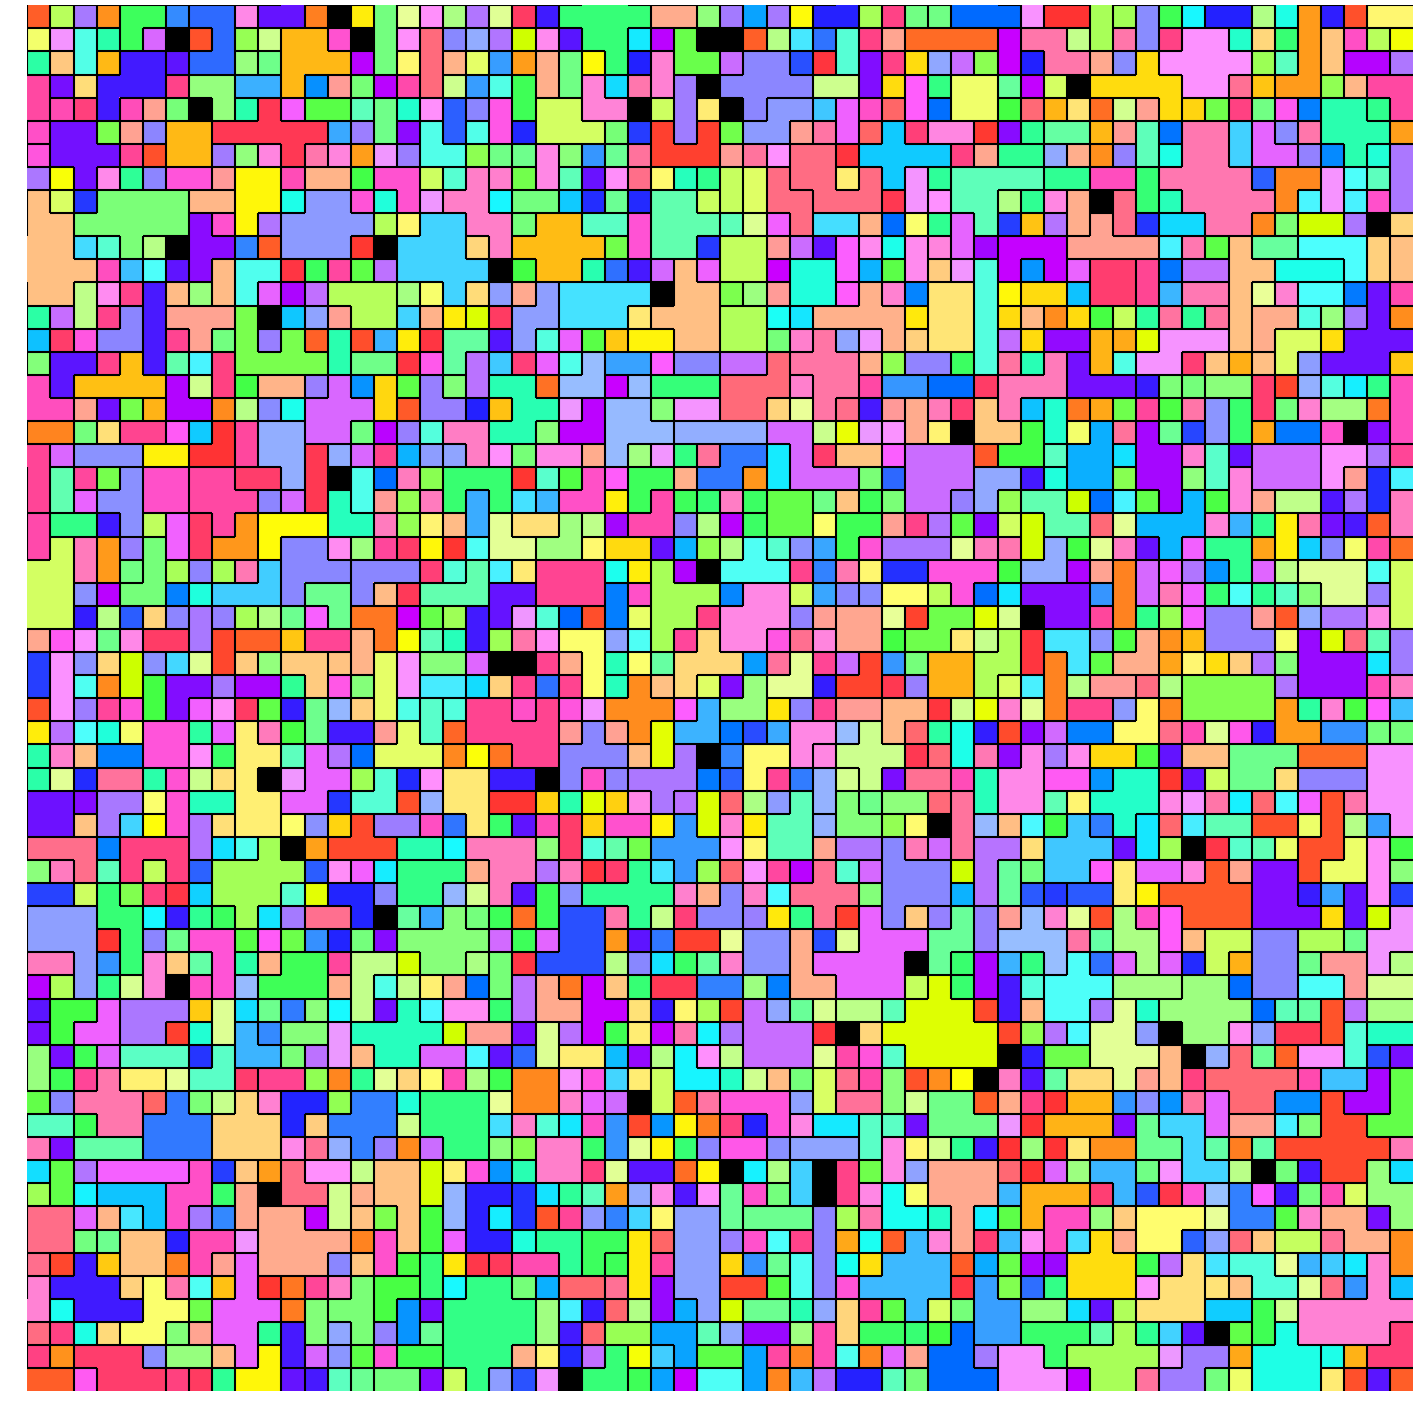
\includegraphics[width=\columnwidth]{seed=1001+title=channel_viz+treat=wave-small__mut-b_medlow+update=50000+_data_hathash_hash=0c0190afbbcd9acb+_script_fullcat_hash=474b4115ecde8750+_source_hash=d53f428-clean+ext=}
\end{subfigure}
\begin{subfigure}[b]{0.45\columnwidth}
  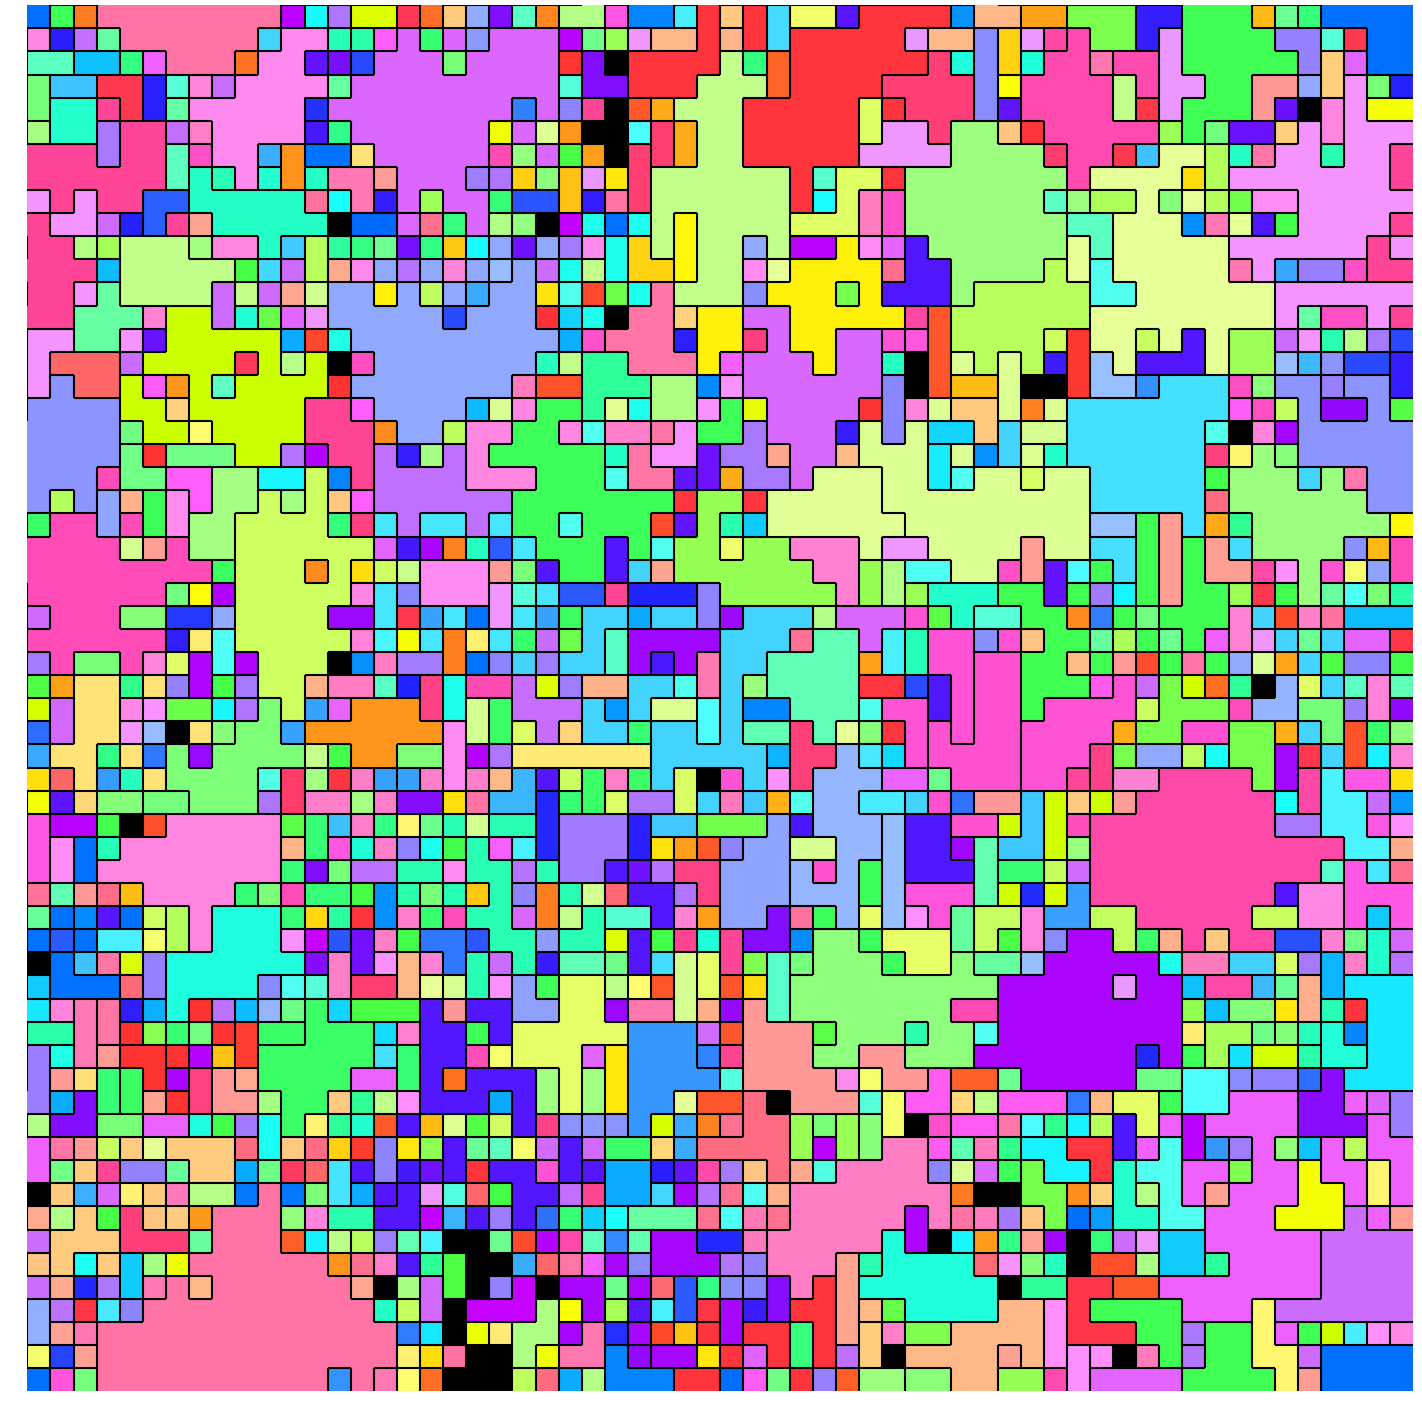
\includegraphics[width=\columnwidth]{seed=1001+title=channel_viz+treat=wave-big__mut-b_medlow+update=50000+_data_hathash_hash=50427fb0ffaf976a+_script_fullcat_hash=474b4115ecde8750+_source_hash=d53f428-clean+ext=}
\end{subfigure}

\rotatebox{90}{~~~~~~~Mutational Load 3}
\begin{subfigure}[b]{0.45\columnwidth}
  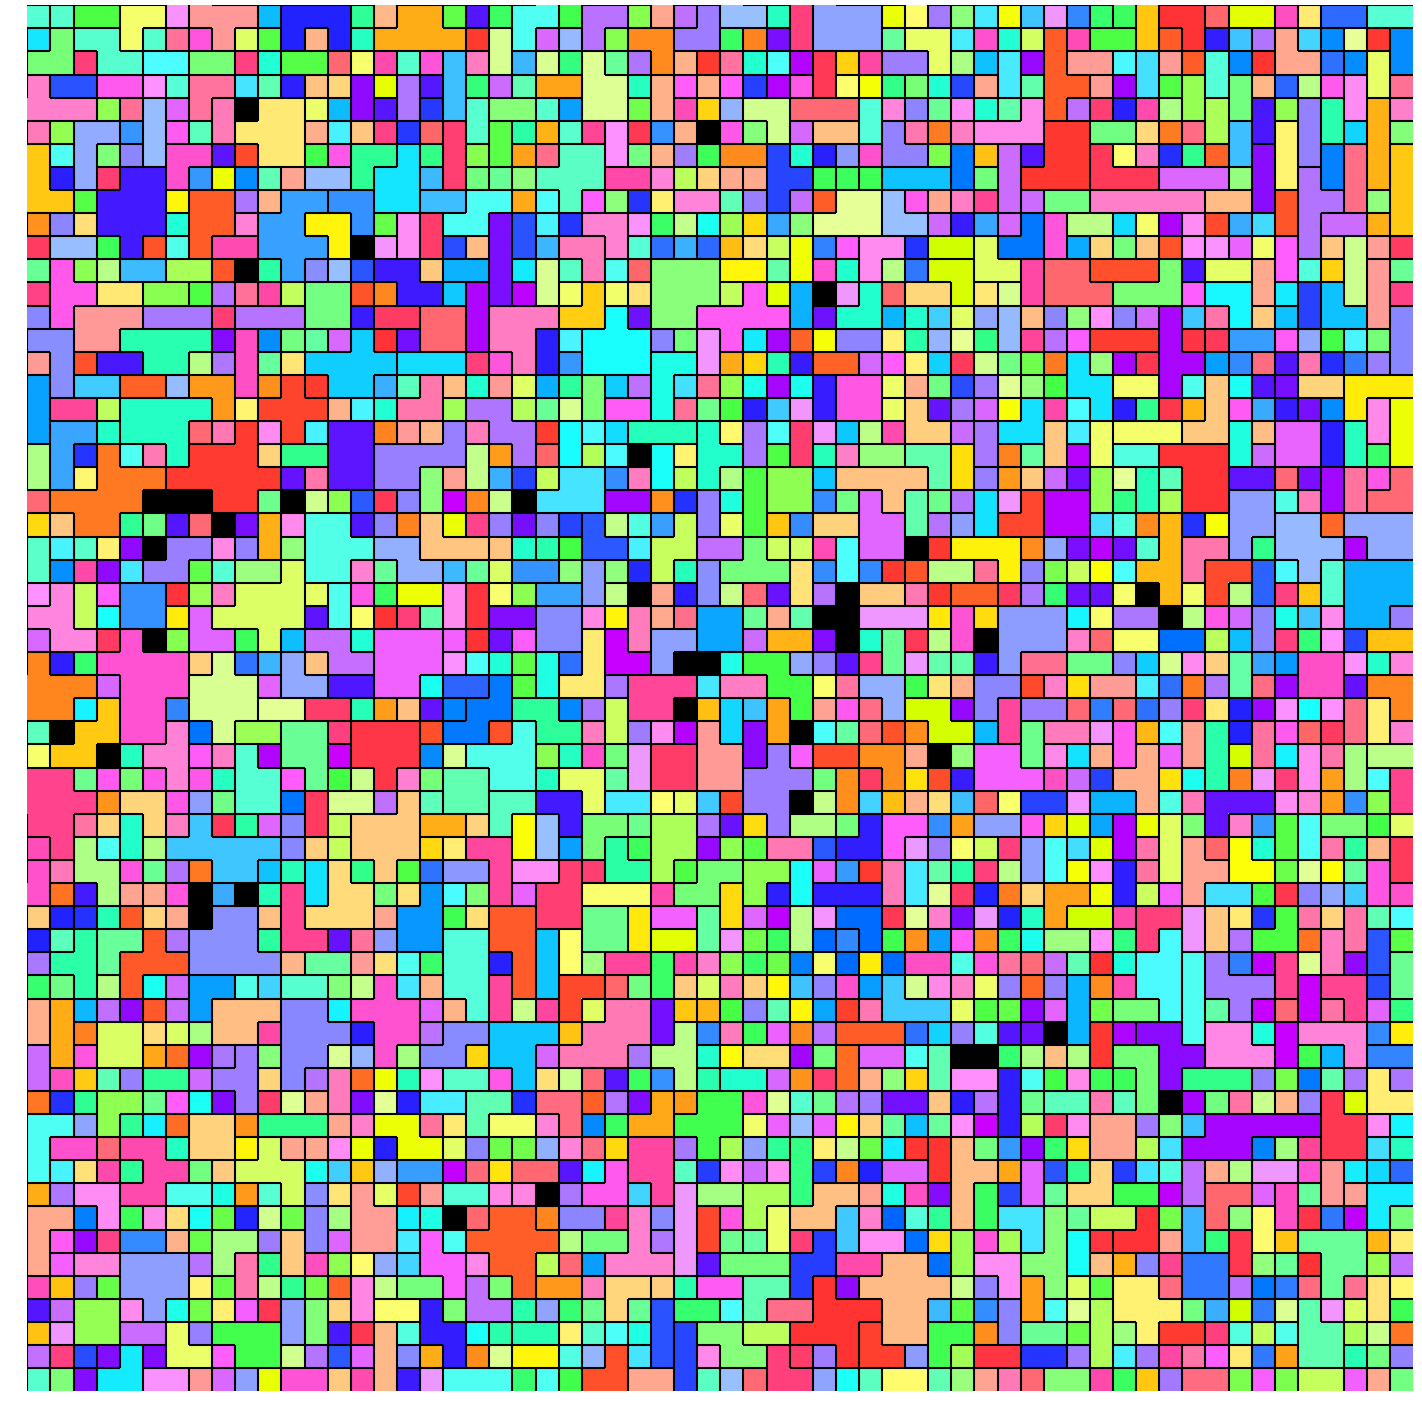
\includegraphics[width=\columnwidth]{seed=1001+title=channel_viz+treat=wave-small__mut-c_medhigh+update=50000+_data_hathash_hash=153e2f8791347e2b+_script_fullcat_hash=474b4115ecde8750+_source_hash=d53f428-clean+ext=}
\end{subfigure}
\begin{subfigure}[b]{0.45\columnwidth}
  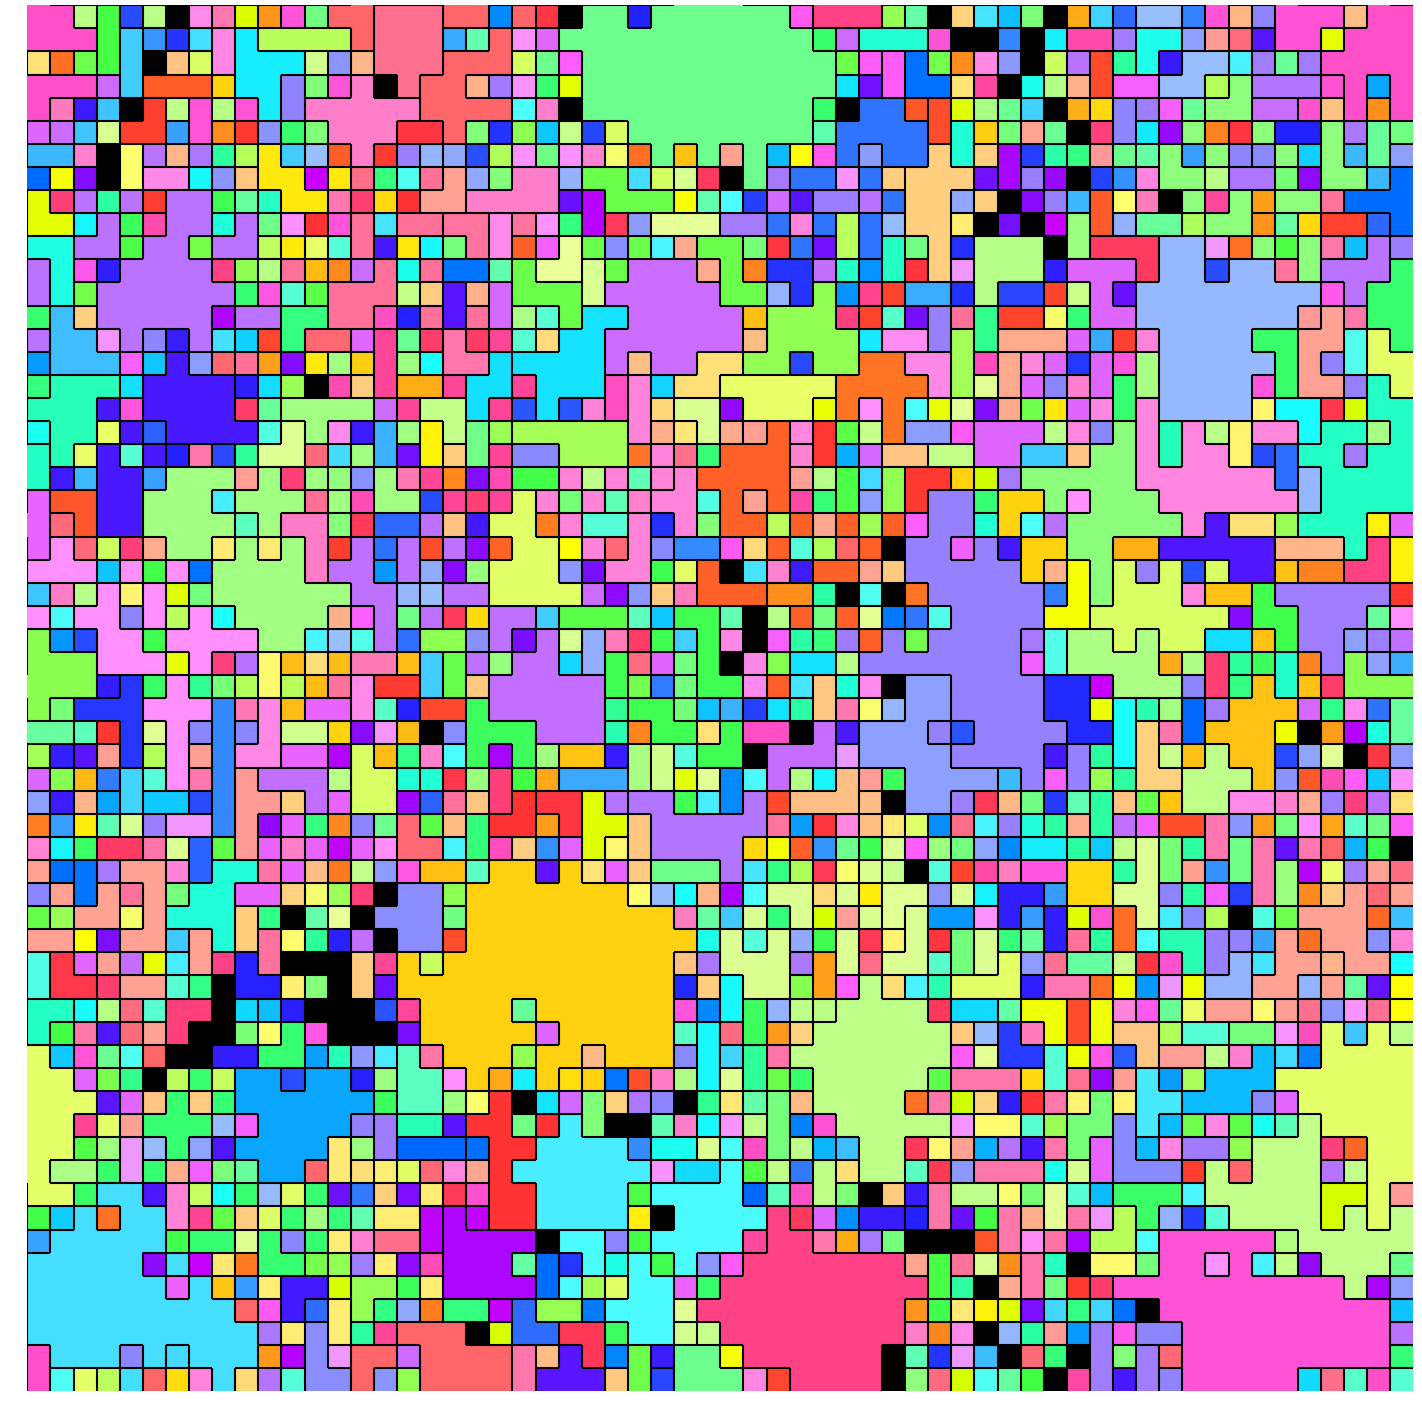
\includegraphics[width=\columnwidth]{seed=1001+title=channel_viz+treat=wave-big__mut-c_medhigh+update=50000+_data_hathash_hash=3bc8464cdb13317c+_script_fullcat_hash=474b4115ecde8750+_source_hash=d53f428-clean+ext=}
\end{subfigure}

\rotatebox{90}{~~~~~~~Mutational Load 4}
\begin{subfigure}[b]{0.45\columnwidth}
  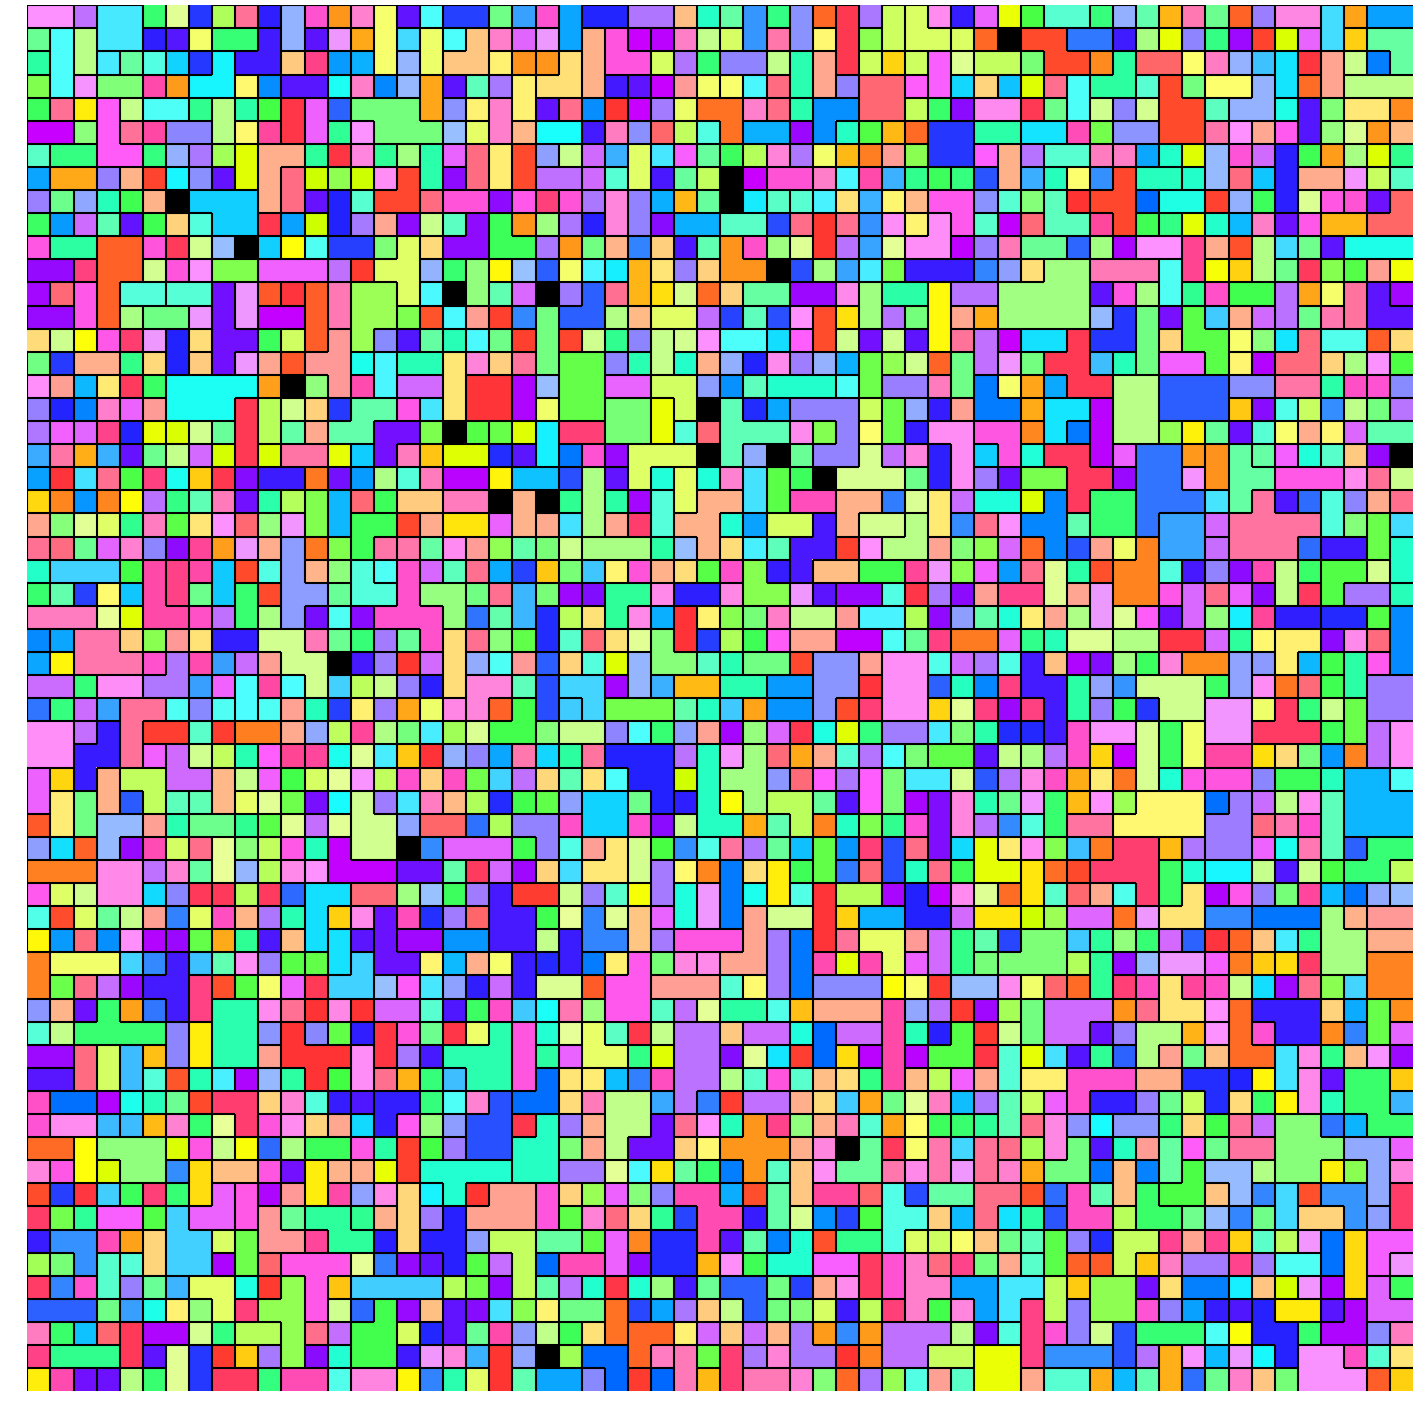
\includegraphics[width=\columnwidth]{seed=1001+title=channel_viz+treat=wave-small__mut-d_high+update=50000+_data_hathash_hash=700947e5ae80d046+_script_fullcat_hash=474b4115ecde8750+_source_hash=d53f428-clean+ext=}
\end{subfigure}
\begin{subfigure}[b]{0.45\columnwidth}
  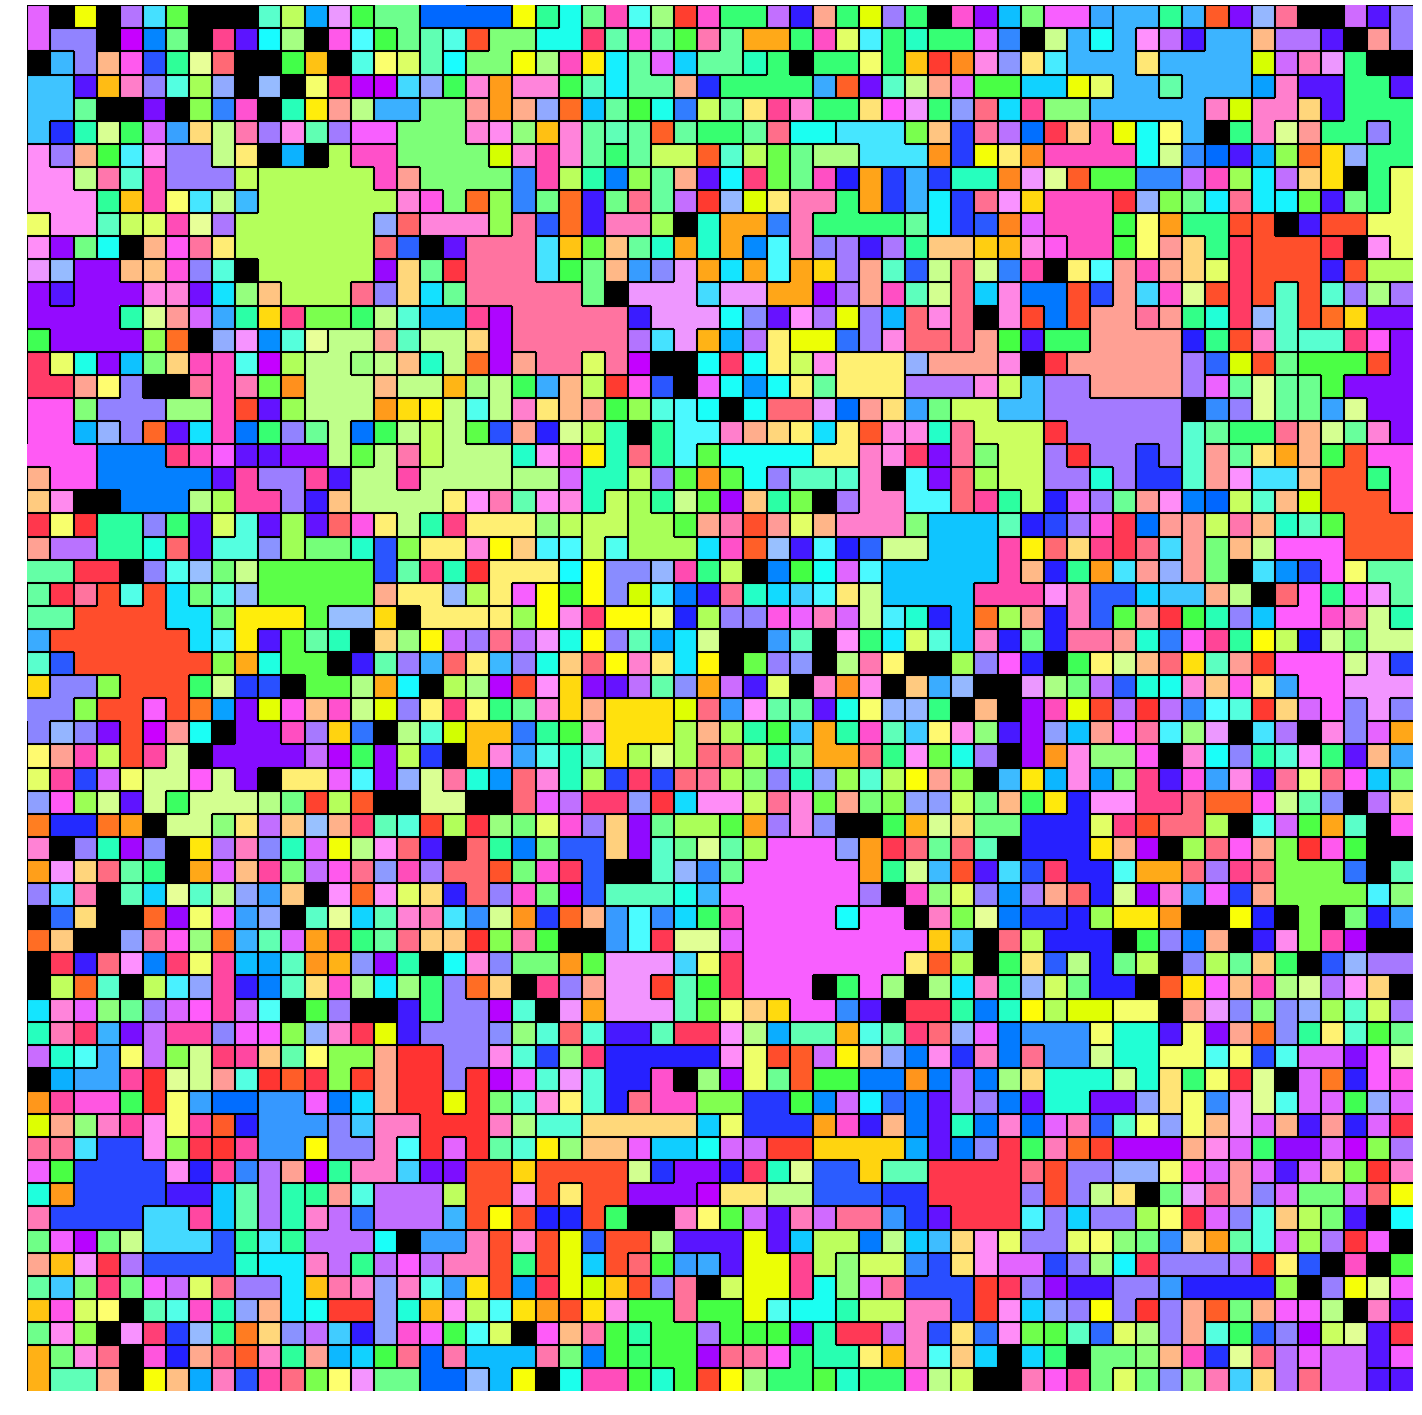
\includegraphics[width=\columnwidth]{seed=1001+title=channel_viz+treat=wave-big__mut-d_high+update=50000+_data_hathash_hash=e7071e390f076a00+_script_fullcat_hash=474b4115ecde8750+_source_hash=d53f428-clean+ext=}
\end{subfigure}

\rotatebox{90}{~~~~~~~Mutational Load 5}
\begin{subfigure}[b]{0.45\columnwidth}
  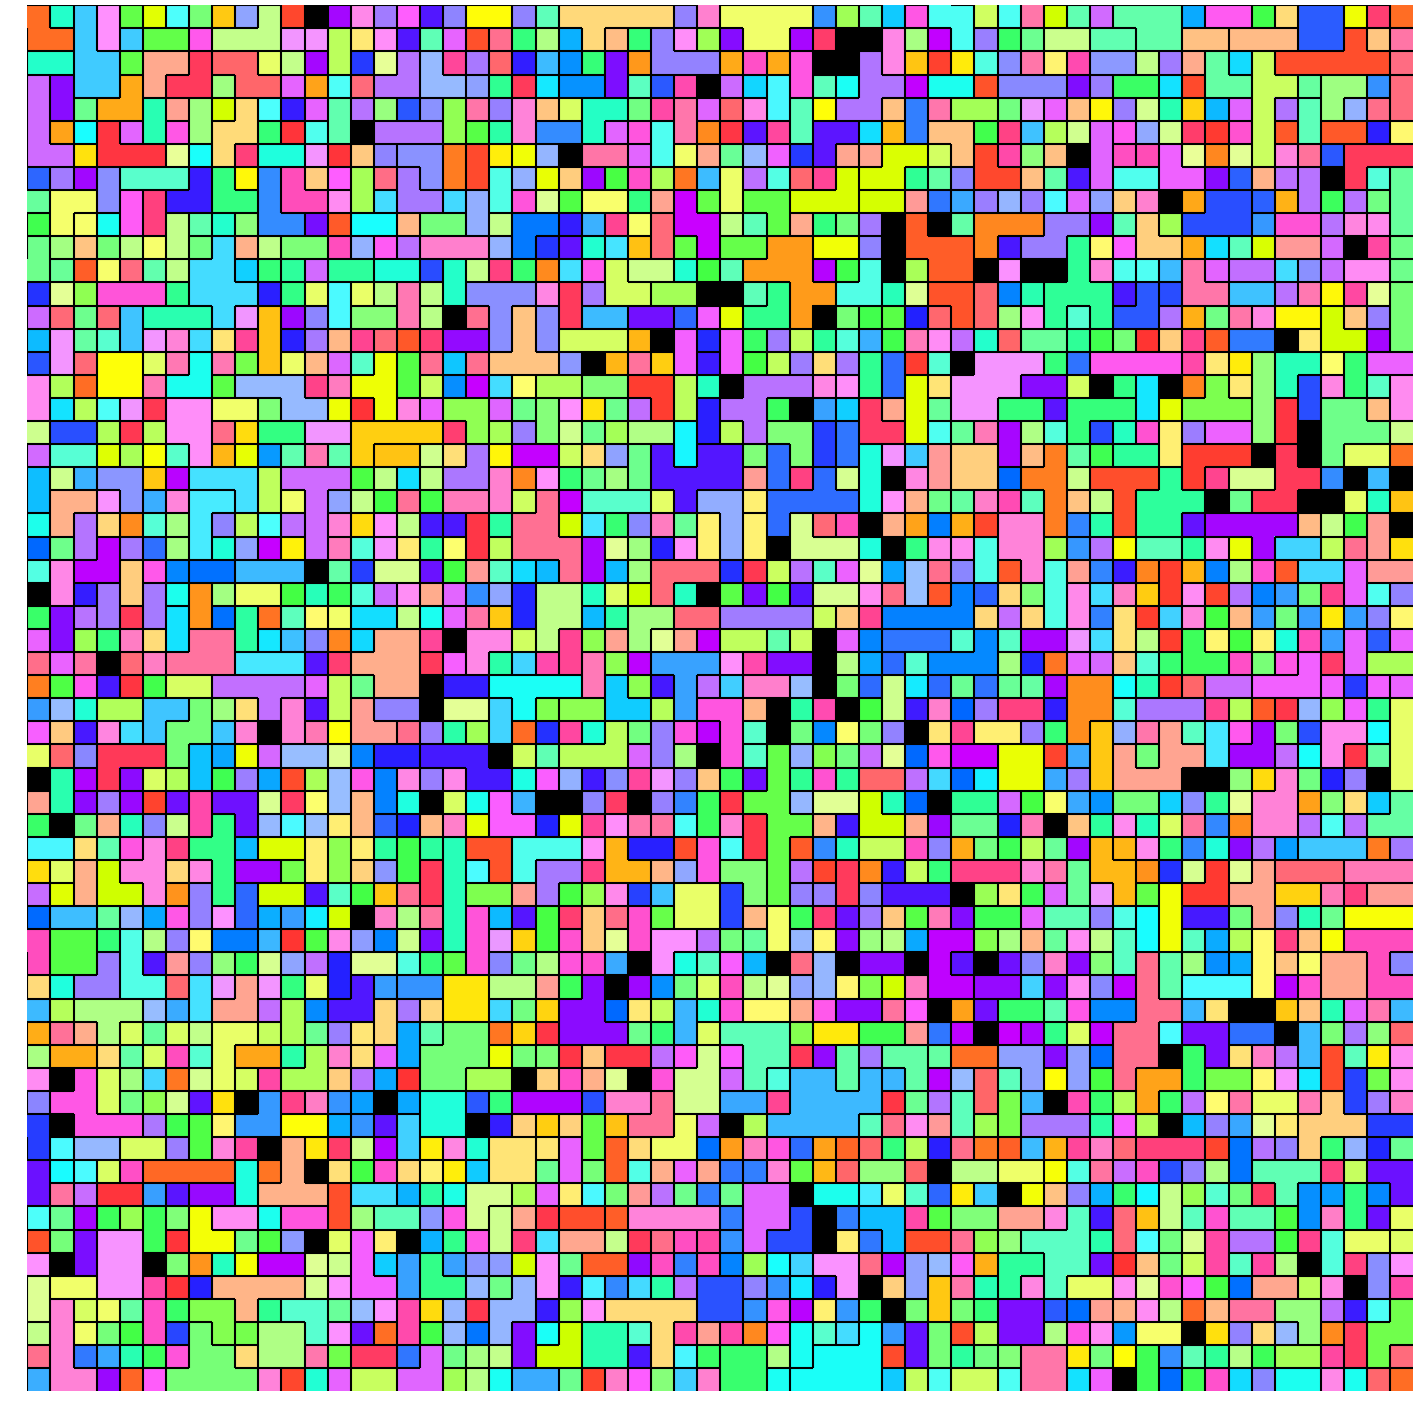
\includegraphics[width=\columnwidth]{seed=1001+title=channel_viz+treat=wave-small__mut-e_extreme+update=50000+_data_hathash_hash=70d59bcccb7f3ca6+_script_fullcat_hash=474b4115ecde8750+_source_hash=d53f428-clean+ext=}
\end{subfigure}
\begin{subfigure}[b]{0.45\columnwidth}
  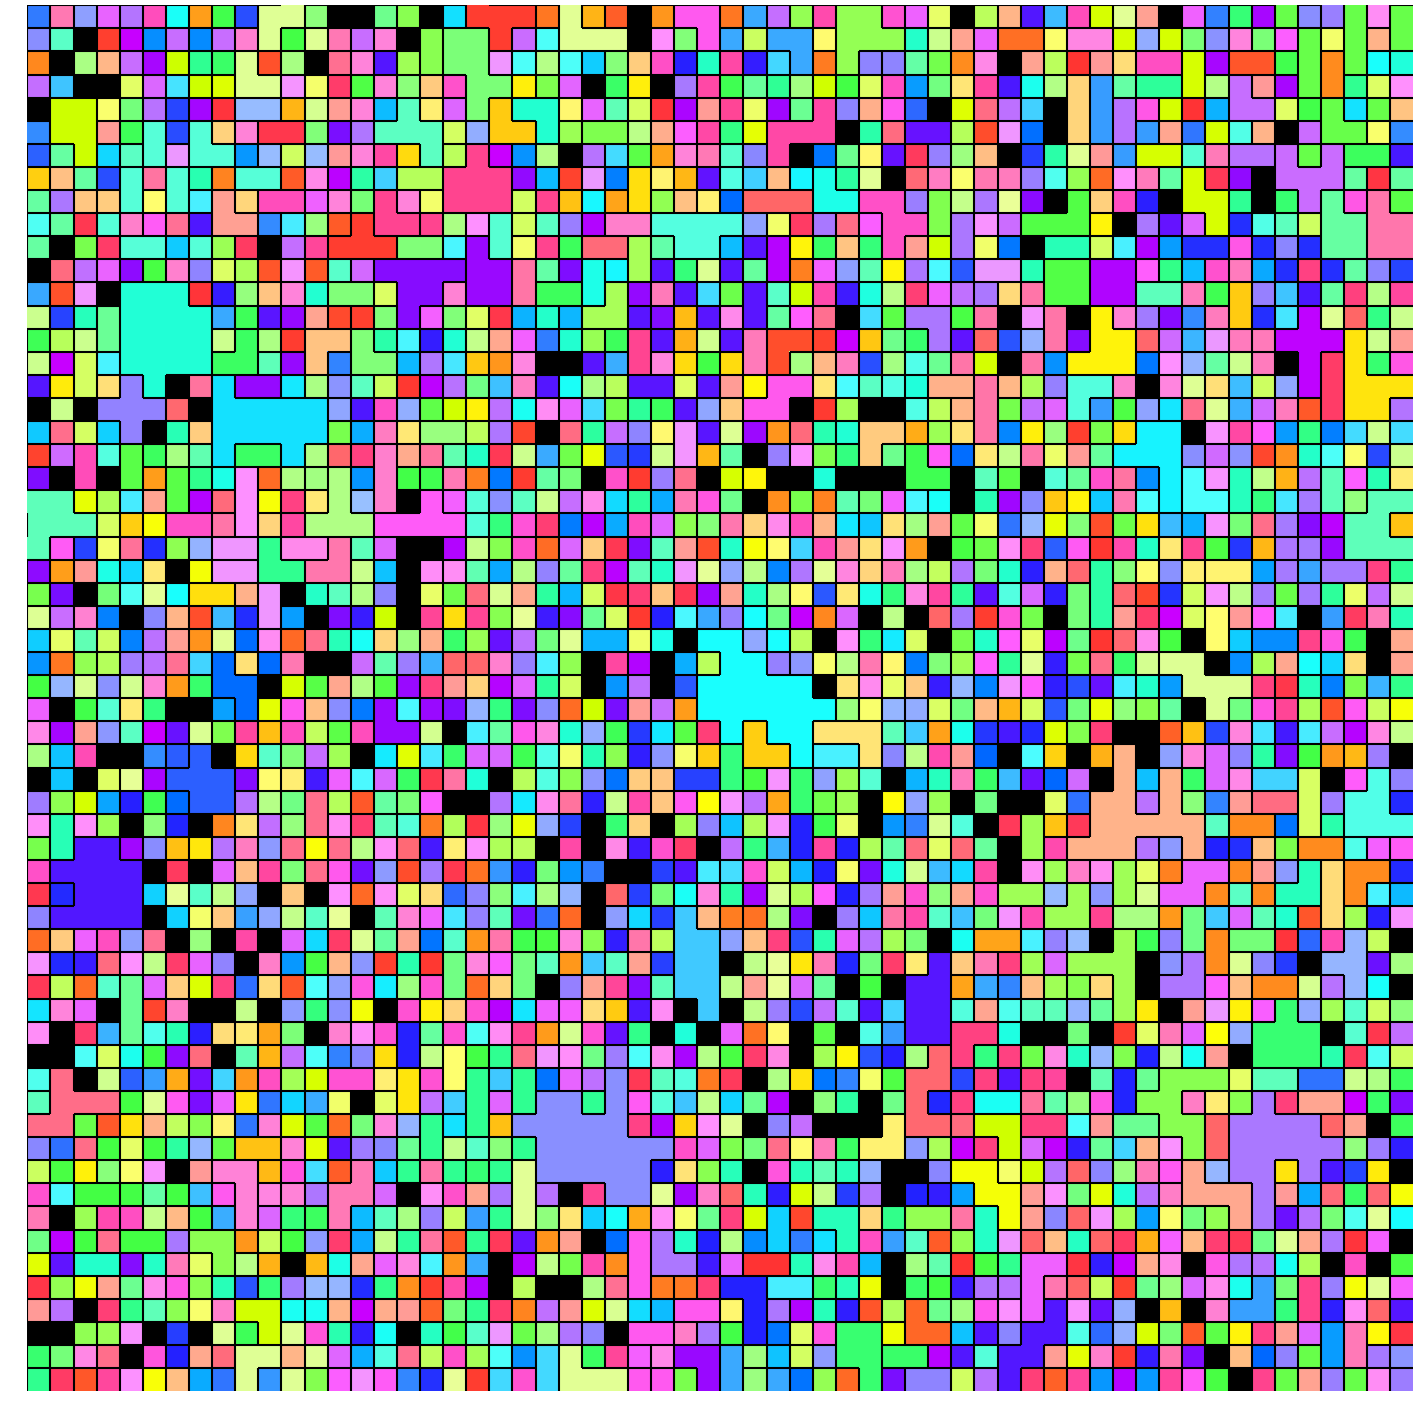
\includegraphics[width=\columnwidth]{seed=1001+title=channel_viz+treat=wave-big__mut-e_extreme+update=50000+_data_hathash_hash=6532b779898a7959+_script_fullcat_hash=474b4115ecde8750+_source_hash=d53f428-clean+ext=}
\end{subfigure}
\caption{
Representative same-channel signaling network end states for runs of each treatment.
A single cell-like organism occupies each grid tile except for black tiles, which are empty.
Channel IDs are coded by color.
Same-channel groups appear as uniformly-colored clumps, bounded by a black border.
}
\label{fig:outcome_grids}
\end{center}
\end{figure}


Indeed, in concordance with this second possibility, in Figure \ref{fig:outcome_grids} we can anecdotally observe more fragmented same-channel groups in treatments with greater mutational load.
This pattern is most strongly apparent in the large resource wave treatments, where the absence of large same-channel groups characteristic of low mutational load is easily observed under high mutational load, but also appears to hold for small resource wave treatments.
A more rigorous, quantitative analysis of this seeming pattern would benefit future work.

\begin{table}
 \centering
 \begin{tabular}{l c|cc} % alignment of each column data
 \multicolumn{4}{c}{\textbf{Extant Phylogenetic Roots}} \\
 & & \multicolumn{2}{c}{Resource Wave Size} \\
 & & Small & Large \\
 \hline
 \multirow{5}{*}{\STAB{\rotatebox[origin=c]{90}{\parbox{1.5cm}{\centering Mutational\\Load}}}} & 1 & $2 \pm 1$ & $61 \pm 52$ \\
 & 2 & $4 \pm 2$ & $80 \pm 51$\\
 & 3 & $5 \pm 1$ & $240 \pm 98$\\
 & 4 & $7 \pm 2$ & $599 \pm 82$\\
 & 5 & $28 \pm 3$ & $1204 \pm 116$\\
\end{tabular}
\caption{
Number of seed genomes with extant descendants (mean $\pm$ standard deviation across replicates).
}
\label{tab:phylogeny_roots}
\end{table}


The number of distinct phylogenetic roots among the extant population at the end of an evolutionary run provides a complimentary measure of evolutionary progress.
If only one phylogenetic root remains at the end of a run, the descendants of a single seeded cell have swept the entire population.
If two remain, the descendants of two distinct seeded cells are represented in the final population.
At the other end of the spectrum, 3600 phylogenetic roots would mean that a descendant from each and every seeded cell is present.
Table \ref{tab:phylogeny_roots} provides this metric for each treatment.
In agreement with Table \ref{tab:cell_generations}, the number of phylogenetic roots is lowest for low mutational load with small resource wave size (e.g., over more cellular generations, selection has eliminated a greater number of phylogenies) and the number of phylogenetic roots is greatest for high mutational load with large resource wave size (e.g., over fewer cellular generations, selection has yet to eliminate as many phylogenies).
From an evolutionary computing practitioner's perspective, the small number of extant phylogenies for low mutational load with small resource wave size --- generally, around two --- suggests that adaptive selection has strongly shaped the population in these replicates by the end of the evolutionary run.
However, the large number of extant phylogenies for high mutational load with large resource wave size --- generally, around 1200 --- suggests that adaptive selection has not as strongly shaped the population in these replicates by the end the of the evolutionary run.

With more computing time, we could extend the evolutionary runs of treatments with large resource wave size and/or larger mutational load in order to obtain populations with comparable evolutionary progress for all treatments.
However, we can still identify and discuss interesting differences between treatments while keeping this complicating factor in mind.

The central question we wish to answer:


\section{Conclusion}

In this work, we showed that high mutational load derails the evolution of cooperative, multicellular phenotypes.
Specifically, we were able to observe,
\begin{itemize}
\item cooperative reproductive behavior observed under low mutational load is replaced by antagonistic reproductive behavior under high mutational load,
\item cooperative resource sharing behavior observed under low mutational load disappears under higher mutational loads,
\item the evolution of cooperative reproductive behavior in numerically large cell groups (e.g., large resource wave treatments) is more sensitive to mutational load than in numerically small cell groups (e.g., small resource wave treatments), and
\item the evolution of resource sharing in small cell groups is more sensitive to mutational load than in large cell groups.
\end{itemize}

Questions remain, especially due to small number of cellular generations elapsed in some treatments.
Performing longer evolutionary runs, at least until descendants from a single seeded genome sweep the population, would provide certainty that our observations --- especially with respect large resource wave treatments --- are not artifacts of small generation counts.
Performing much longer evolutionary runs would provide another opportunity: to look for the evolution of behaviors that counteract mutational load so that cooperative strategies can succeed despite mutation load.
Biological multicellular organisms have evolved mechanisms to manage somatic mutation and, especially, reduce the incidence of malignant mutants (e.g., cancer).
Strategies include genetic pathways that induce a cell to destroy itself in response to genetic damage \citep{lee1995apoptosis} and immune responses where other cells recognize and destroy malignant cells \citep{Martinez-Lostao5047}.
To attempt to evolve strategies to counteract mutational load we might begin with a population under low mutational load where cooperative behavior evolves and then gradually increase mutational load.
If cooperative behavior remains at mutational loads where it does not spontaneously evolve, this might suggest the presence of mutation-fighting adaptation.
The mechanism of such an adaptation might be of scientific or practical interest.

DISHTINY is designed with in a distributed framework in which individual digital cells operate independently and periodically communicate with neighbors via messages.
Hence, it can scale as additional computing resources are provided.
Parallel computing is widely exploited in evolutionary computing, where subpopulations are farmed out for periods of isolated evolution or single genotypes are farmed out for fitness evaluation
\citep{lin1994coarse, real17a}.
DISHTINY presents a more fundamental parallelization potential: principled parallelization of the evolving individual phenotype at arbitrary scale (i.e., a high-level individual as a large collection of individual cells distributed across processing elements).
Such parallelization will be key to realizing evolving computational systems with scale --- and, perhaps, complexity --- approaching those of biological systems.
From an applied perspective, such distributed systems might enable the evolution of more complex digital organisms that exhibit more sophisticated, and potentially useful, capabilities (for example, as reinforcement-learning agents).
From a scientific perspective, we believe that as an experimental platform large-scale digital multicellularity will yield unique insight into questions raised by theoretical evolutionary biology with respect to evolutionary transitions in individuality.


\section{Acknowledgements}

Thanks to members of the DEVOLAB, in particular Charles Ofria for help detangling complicated results and Alexander Lalejini for help with navigating the SignalGP API and graphically depicting SignalGP.
This research was supported in part by NSF grants DEB-1655715 and DBI-0939454, and by Michigan State University through the computational resources provided by the Institute for Cyber-Enabled Research.
This material is based upon work supported by the National Science Foundation Graduate Research Fellowship under Grant No. DGE-1424871.
Any opinions, findings, and conclusions or recommendations expressed in this material are those of the author(s) and do not necessarily reflect the views of the National Science Foundation.


\footnotesize
\bibliographystyle{apalike}
\bibliography{bibl} % replace by the name of your .bib file


\end{document}
